\documentclass{article}[18pt]
\ProvidesPackage{format}
%Page setup
\usepackage[utf8]{inputenc}
\usepackage[margin=0.7in]{geometry}
\usepackage{parselines} 
\usepackage[english]{babel}
\usepackage{fancyhdr}
\usepackage{titlesec}
\hyphenpenalty=10000

\pagestyle{fancy}
\fancyhf{}
\rhead{Sam Robbins}
\rfoot{Page \thepage}

%Characters
\usepackage{amsmath}
\usepackage{amssymb}
\usepackage{gensymb}
\newcommand{\R}{\mathbb{R}}

%Diagrams
\usepackage{pgfplots}
\usepackage{graphicx}
\usepackage{tabularx}
\usepackage{relsize}
\pgfplotsset{width=10cm,compat=1.9}
\usepackage{float}

%Length Setting
\titlespacing\section{0pt}{14pt plus 4pt minus 2pt}{0pt plus 2pt minus 2pt}
\newlength\tindent
\setlength{\tindent}{\parindent}
\setlength{\parindent}{0pt}
\renewcommand{\indent}{\hspace*{\tindent}}

%Programming Font
\usepackage{courier}
\usepackage{listings}
\usepackage{pxfonts}

%Lists
\usepackage{enumerate}
\usepackage{enumitem}

% Networks Macro
\usepackage{tikz}


% Commands for files converted using pandoc
\providecommand{\tightlist}{%
	\setlength{\itemsep}{0pt}\setlength{\parskip}{0pt}}
\usepackage{hyperref}

% Get nice commands for floor and ceil
\usepackage{mathtools}
\DeclarePairedDelimiter{\ceil}{\lceil}{\rceil}
\DeclarePairedDelimiter{\floor}{\lfloor}{\rfloor}

% Allow itemize to go up to 20 levels deep (just change the number if you need more you madman)
\usepackage{enumitem}
\setlistdepth{20}
\renewlist{itemize}{itemize}{20}

% initially, use dots for all levels
\setlist[itemize]{label=$\cdot$}

% customize the first 3 levels
\setlist[itemize,1]{label=\textbullet}
\setlist[itemize,2]{label=--}
\setlist[itemize,3]{label=*}

% Definition and Important Stuff
% Important stuff
\usepackage[framemethod=TikZ]{mdframed}

\newcounter{theo}[section]\setcounter{theo}{0}
\renewcommand{\thetheo}{\arabic{section}.\arabic{theo}}
\newenvironment{important}[1][]{%
	\refstepcounter{theo}%
	\ifstrempty{#1}%
	{\mdfsetup{%
			frametitle={%
				\tikz[baseline=(current bounding box.east),outer sep=0pt]
				\node[anchor=east,rectangle,fill=red!50]
				{\strut Important};}}
	}%
	{\mdfsetup{%
			frametitle={%
				\tikz[baseline=(current bounding box.east),outer sep=0pt]
				\node[anchor=east,rectangle,fill=red!50]
				{\strut Important:~#1};}}%
	}%
	\mdfsetup{innertopmargin=10pt,linecolor=red!50,%
		linewidth=2pt,topline=true,%
		frametitleaboveskip=\dimexpr-\ht\strutbox\relax
	}
	\begin{mdframed}[]\relax%
		\centering
		}{\end{mdframed}}



\newcounter{lem}[section]\setcounter{lem}{0}
\renewcommand{\thelem}{\arabic{section}.\arabic{lem}}
\newenvironment{defin}[1][]{%
	\refstepcounter{lem}%
	\ifstrempty{#1}%
	{\mdfsetup{%
			frametitle={%
				\tikz[baseline=(current bounding box.east),outer sep=0pt]
				\node[anchor=east,rectangle,fill=blue!20]
				{\strut Definition};}}
	}%
	{\mdfsetup{%
			frametitle={%
				\tikz[baseline=(current bounding box.east),outer sep=0pt]
				\node[anchor=east,rectangle,fill=blue!20]
				{\strut Definition:~#1};}}%
	}%
	\mdfsetup{innertopmargin=10pt,linecolor=blue!20,%
		linewidth=2pt,topline=true,%
		frametitleaboveskip=\dimexpr-\ht\strutbox\relax
	}
	\begin{mdframed}[]\relax%
		\centering
		}{\end{mdframed}}
\lhead{Software Engineering - Modelling and Analysis}


\begin{document}
\begin{center}
\underline{\huge Viewpoints and Models}
\end{center}
\begin{itemize}
	\item Any notation we use, whether diagrammatic or mathematical/textual, has to try to balance the following (largely conflicting objectives)
	\begin{itemize}
		\item To provide a description that is sufficiently abstract for the particular task, so that unnecessary detail is omitted
		\item To provide enough detail that it is possible to reason about the model, in order to perform the tasks at hand
	\end{itemize} 
	\item The design process generally involves considerable degrees of 'trade-off' between these needs
\end{itemize}
\section{Hierarchy}
\begin{itemize}
	\item Having forms of notation that can be used in a hierarchical manner can help reduce cognitive load
	\item This permits a description of an element at one level to be expanded into one that employs the same form, but a set of less abstract elements, at a lower level
\end{itemize}
\section{Modelling and Architecture}
Architectural ideas present two problems
\begin{itemize}
	\item It's quite hard to model the forms of different architectural designs themselves, although attempts have been made
	\item Many modelling notations, particularly those concerned with modelling the structure of a system, do implicitly assume the use of some specific form of architecture. This is particularly true for object-oriented modelling (class diagrams) and call-and-return too
	\item This is less true when modelling behaviour or state, where our models rarely assume the use of particular types of software elements
\end{itemize}
\section{The functional viewpoint}
\begin{itemize}
	\item Describes the actions and operations that are to be performed by a system
	\item The way that this is described may well depend on the architectural style(s) being used
	\begin{itemize}
		\item In a Dataflow style, would expect to model function in terms of operations and information flow
		\item In a Call-and-Return style might expect to be concerned about the sequencing of actions
	\end{itemize}
	\item In practice, this is one of the hardest viewpoints to capture, partly because of the influence of the architectural style, and also because function can be hard to model with a diagrammatic form
\end{itemize}
\subsection{The Data Flow Diagram (DFD)}
\begin{itemize}
	\item Essentially a problem-oriented (black box) form used extensively for modelling application functionality
	\item Traditionally used in the process of the Structured Systems Analysis/Structured Design family of plan-driven design methods, which progress from a Data Flow 'black box' analysis model to a Call-and-Return 'white-box' implementation form
\end{itemize}
\subsubsection{The DFD Symbols}
\begin{center}
	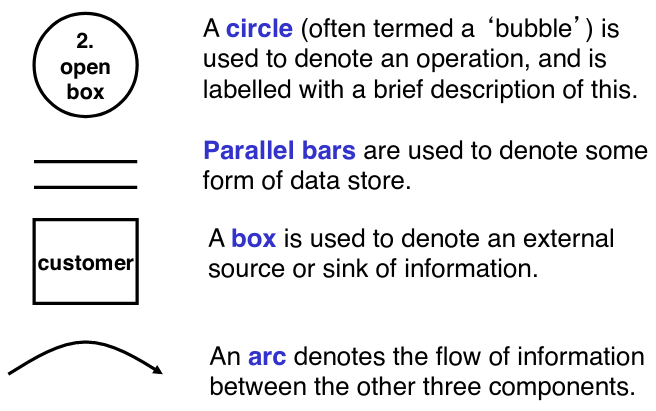
\includegraphics[scale=0.7]{DFD-Symbols}
\end{center}
\subsubsection{The context diagram}
\begin{itemize}
	\item This is the very top level of a DFD, consisting of a single bubble (to represent the system) and a set of sinks and sources
\end{itemize}
\begin{center}
	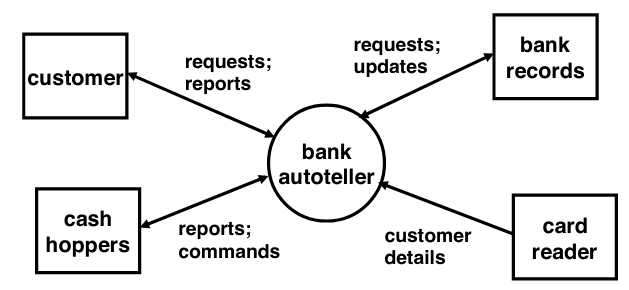
\includegraphics[scale=0.7]{Context-Diagram}
\end{center}
\subsubsection{Hierarchy in DFDs}
\begin{itemize}
	\item The Context Diagram is then expanded into a top level DFD that describes the overall system operation
	\item DFDs are hierarchical in form, in that bubbles can be expanded by using a further diagram that shows the details of an operation as a DFD
	\item Convention is to use a numbering system with 1 at the top 1.1... at the next level and 1.1.1... at the next
\end{itemize}
\subsection{A top-level DFD}
\begin{center}
	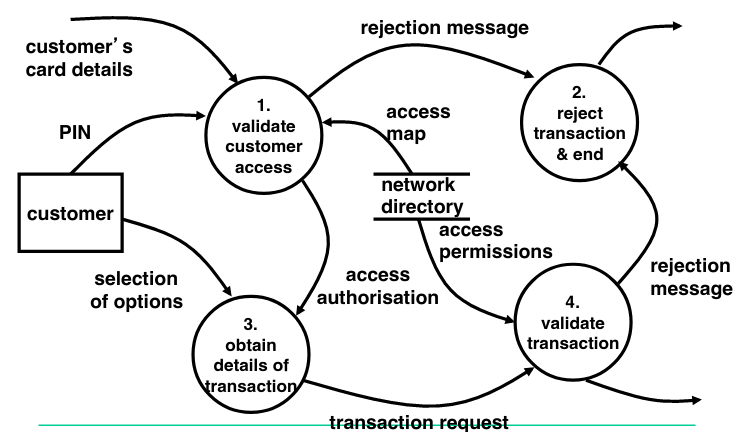
\includegraphics[scale=0.7]{top-level-dfd}
\end{center}
\subsection{What not to include}
\begin{itemize}
	\item A DFD does not include details of the control flow that may be involved in operations
	\item Also, we try to limit the descriptions to be brief
\end{itemize}
\subsubsection{Usefulness}
\begin{itemize}
	\item Regardless of the form of 'solution' we are seeking DFDs can still be useful for modelling some of the aspects of how an application is to work
	\item In particular, they have the benefit that they can quite easily be explained to customers, and used to help ensure that there is a common understanding of what an application is to do
	\item Can be useful for identifying user stories, which we often employ during agile development
\end{itemize}
\subsection{The activity diagram}
Activity diagrams are often used to model the way that a business operates. Like DFDs, they focus on describing how information flows through a system and gets transformed, but do so by modelling events. Some key notational elements are:
\begin{center}
	\includegraphics[scale=0.7]{"activity diagram"}
\end{center}
\section{The behavioural viewpoint}
\begin{itemize}
	\item Used to capture casual issues through the use of the notion of a finite state machine
	\item Models for this viewpoint tend to be abstractions that are concerned with states and events and with identifying the transitions that can occur between the different states
\end{itemize}
\subsection{State Transition Diagram (STD)}
Can be used fo "finite state machine" modelling of
\begin{itemize}
	\item "system" behaviour at the top level (black box)
	\item the detailed behaviour of design entities
\end{itemize}
Various notations - this has four main elements
\begin{itemize}
	\item Labelled box to denote state
	\item Arc to denote a transition
	\item Text above line for the transition condition
	\item Text below line for transition action
\end{itemize}
Does not readily scale up for large systems, as the lack of any hierarchical element means that there is no means of expressing groupings of states
\subsection{State Transition Table (STT)}
Particularly useful when:
\begin{itemize}
	\item Checking for a completeness of a design model
	\item Developing the state model, as it may be useful to tabulate the information first, and then draw the diagram
\end{itemize} 
Lacks the ready visualisation of an STD, but handles scale much better, although still non-hierarchical\\
\\
Provokes thinking about the "non-events" such as when a user does something unexpected

\end{document}